\documentclass[conference, letterpaper, 10pt, times]{IEEEtran}

%% IEEE CNS addition:
\makeatletter
\def\ps@headings{%
	\def\@oddhead{\mbox{}\scriptsize\rightmark \hfil \thepage}%
	\def\@evenhead{\scriptsize\thepage \hfil \leftmark\mbox{}}%
	\def\@oddfoot{}%
	\def\@evenfoot{}}
\makeatother
\pagestyle{empty}

\usepackage[T1]{fontenc}

\usepackage[dvipsnames]{xcolor}
\usepackage{graphicx}

\usepackage[binary-units]{siunitx}
\sisetup{range-phrase=--, range-units=single}

\usepackage[basic]{complexity}
\usepackage[super,negative]{nth}

\usepackage{booktabs}
\usepackage{microtype}

%% Fix indent in new section...
\newcommand{\subparagraph}{}
\usepackage{titlesec}
\titlespacing*{\section}{0pt}{1.5ex}{0.7ex}
%\titleformat*{\filcenter\scshape}

%bib
\usepackage[maxnames=3,maxbibnames=99,mincrossrefs=5,style=ieee,sortcites,backend=bibtex]{biblatex}
\addbibresource{papers-off.bib}
\addbibresource{confs-off.bib}
\addbibresource{books-off.bib}
\addbibresource{rfc.bib}
\addbibresource{misc.bib}

%picky abt et al.
\usepackage{xpatch}

\xpatchbibmacro{name:andothers}{%
	\bibstring{andothers}%
}{%
	\bibstring[\emph]{andothers}%
}{}{}

%opening!

\newcommand{\mytitle}{Improving Direct-Control Reinforcement Learning for Network Intrusion Prevention}

\usepackage{url}
\usepackage{hyperref}
\usepackage{cleveref}
\newcommand{\crefrangeconjunction}{--}

\hypersetup{
	colorlinks,
	citecolor=black,
	filecolor=black,
	linkcolor=black,
	urlcolor=black,
	pdftitle={\mytitle{}},
	pdfauthor={Kyle A. Simpson}
}
\newcommand*{\email}[1]{\href{mailto:#1}{\nolinkurl{#1}} } 

\usepackage{titling}
\settowidth{\thanksmarkwidth}{*}
\setlength{\thanksmargin}{-\thanksmarkwidth}

%% Enable /thanks
\IEEEoverridecommandlockouts
\makeatletter
\def\footnoterule{\relax%
	\kern-5pt
	\hbox to \columnwidth{\hfill\vrule width 0.5\columnwidth height 0.4pt\hfill}
	\kern4.6pt}
\makeatother

%-------------------------------------%
%-------------------------------------%

\title{\mytitle{}}
\author{Kyle A. Simpson\thanks{This work was supported by the Engineering and Physical Sciences
		Research Council [grant number EP/M508056/1]}\\\emph{University of Glasgow, Glasgow, Scotland},\\
		\email{k.simpson.1@research.gla.ac.uk}}

% Remove date, leave no spacing.
\predate{}
\postdate{}
\date{}

\begin{document}

%% If needed, make urls typewritery
%\urlstyle{tt}

\maketitle

\begin{abstract}
Network intrusion detection and prevention systems backed by machine learning (and the autonomous operation they promise) have been long-heralded, but face problems hampering effective deployment.
The detection problem in this domain is fraught with difficulty; it is an evolving, non-stationary problem as usage patterns shift, new protocols and applications are introduced, compounded by burstiness and seasonal variation.

\emph{Reinforcement learning} (RL) may overcome the detection problem for certain classes of anomaly by managing and monitoring \emph{consequences}; an agent's role is to learn to optimise performance criteria (which are always available).

I present...
?? Contribs

?? Taking up space to figure out how much room I have for an intro

?? still taking up space...

?? still going...

?? done...
\end{abstract}

\section{Introduction}

What is the story I'm trying to push?

?? Threat model yada yada everything sucks all the time here are some statistics about things being 

?? Reference to the possible mistreatment of RL in our domain? The problem of ``blind application'' so hated by \textcite{DBLP:conf/sp/SommerP10}.

?? RL as a mechanism to protect systems by monitoring performance characteristics---overcome the detection problem (different handle on the key problems of burstiness, evolution, non-stationarity).

This paper contributes:
\begin{itemize}
	\item A DDoS mitigation system based on direct-control reinforcement learning designed for deployment in real-world software-defined networks.
	\item Important weaknesses and flaws in the past design and evaluation of similar techniques \cite{DBLP:journals/eaai/MalialisK15}---deconstruction of the ISP-like formulation, an acknowledgement of the flaws and risk factors of pushback \cite{DBLP:journals/ccr/MahajanBFIPS02a}.
	\item ?? TODO: Advancing the use/representation of state-space in direct-control RL of networked applications.
\end{itemize}

\section{Background}

%?? Introduce RL, related definitions etc.
\emph{Reinforcement learning} (RL) is a variant of machine learning principally concerned with with training an agent to perform optimally in the pursuit of a given task \cite{RL2E}.
We assume the agent has a certain amount of knowledge whenever a decision must be made: at any point in time it knows which \emph{state} it is in, the set of \emph{actions} which are available to it, and a numeric \emph{reward} obtained from the last action chosen if available.
RL methods use this information to gradually refine their \emph{valuation} of states or state-action pairs---allowing the inference of policies which choose actions to maximise the total reward.

?? Formalise?

?? Include some details of function approximation in the formalisation?

There exists immense variation in \emph{how} policies and values may be learned, reliant upon the particular convergence guarantees required.

?? Is this \emph{actually} just sarsa? We're using fn approx (of course), but this is fraught with its own difficulties. Is it strictly speaking correct to describe it as Sarsa at this point? It's, at the very least, 1-step semi-gradient Sarsa given that it is clearly on-policy...
?? IDEA: try out average reward, td($\lambda$) methods...

?? Discuss mininet? Networking terms? SDN stuff?

\section{A Plan, of Sorts}

\begin{enumerate}
	\item The main case for contribution in what I have so far:
	\begin{itemize}
		\item Past work reliant on unrealistic network models: tcp-like behaviour (and its effects on collateral damage) not captured, disjoint ranges of traffic distribution (no benign heavy-hitters), ISP-like topology.
		\item I offer more realistic network emulation environment, better treatment of protocol/traffic characteristics.
	\end{itemize}
	\item Forthcoming: rethinking state/action spaces to operate at a finer level of granularity. New network model (live tcp back-and-forth), allows us to test collateral damage assumptions in a more realistic manner (and show clear case for moving beyond work of malialis and kudenko)
\end{enumerate}

\section{Methodology}

?? Either say ``I did it like \textcite{DBLP:journals/eaai/MalialisK15}, here are the differences (i.e., the \emph{real} innovations)'' or just spend time going over it again.

?? STRUCTURE: Either (methodology) -> (results) OR (their stuff + its weaknesses) -> (a new direction) [second is way punchier, but not yet ready to go with that.]

\section{Results and Evaluation}

\begin{figure}[ht]
	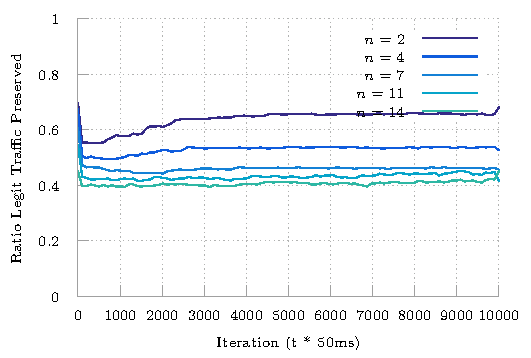
\includegraphics[width=\linewidth]{../plots/online-varyN-uneven}
	\caption{
		MARL pushback control system performance plotted over time, for various settings of $n$ hosts per learner.
		This plot shows that, from the perspective of benign hosts, service guarantees degrade as inference and applied actions become less granular.
		This generalises for all behavioural discriminators: even a perfect agent \emph{must} punish benign flows if they are grouped with malicious actors.
		\label{fig:marl-granularity}
	}
\end{figure}

See above: a result.

?? Observations: training time lengthier by nature of emulated environment.
?? Risk of going for a simulation (i.e. numeric)? Always going to be interesting behaviour that is missed out on (in theory), at the cost of training time/limits of simulation speed

\section{Related Work}

?? Other recent work in the prevention of DDoS? (i.e., non-RL).

%?? Abuses of RL 
Earnest, well-considered application of RL towards the challenge of intrusion detection/prevention has seen comparatively little examination.
Past work exhibits abuses of the paradigm as a glorified classifier for anomaly detection \cite{shamshirband2014anomaly} and DDoS prevention \cite{DBLP:conf/mates/ServinK08}.

?? Good Direct-control work \cite{DBLP:phd/ethos/Malialis14, DBLP:journals/eaai/MalialisK15}

?? Indirect-control applications: link to all the juicy stuff in e.g. HotNets, data-driven networking, the works. \cite{DBLP:conf/hotnets/ValadarskySST17, DBLP:conf/hotnets/MaoAMK16}.
The HMM stuff---learning when best to \emph{communicate} and share knowledge between explicit detector models \cite{DBLP:conf/paisi/XuSH07}.
The latter example's position is slightly weakened by its reliance on the discredited `DARPA99' dataset \cite{DARPA-IDD, DBLP:conf/cisda/TavallaeeBLG09, DBLP:conf/sp/SommerP10}, but the idea itself is well-treated and this acts as a driver for improvements in this direction.

\section{Conclusion}

It all ends here, Mr.\ Bond...

?? Please write me once everything else is in place.

?? Future Work? I.e., \emph{everything}: no one else is really looking at/interested in this specific kind of application of RL yet. \emph{Yet}.

\section*{Acknowledgements}
My thanks go to Dr.\ Dimitrios Pezaros for his supervision, guidance, and comments relating to the realisation of this work.
Additional thanks \emph{would} go out to my anonymous reviewers, had I any of them.

\printbibliography

\end{document}